\chapter{Desarrollo Teórico y Simulaciones}

\section{Fundamento Teórico del Índice Horario}

El índice horario es un parámetro de diseño normalizado que describe el desfase angular existente entre las tensiones
homólogas del bobinado de alta tensión y el bobinado de baja tensión de un transformador trifásico. Dado que las
conexiones trifásicas introducen desfases que son siempre múltiplos de $30^\circ$, se adopta la analogía de la esfera
de un reloj de doce horas. En esta representación, el vector de tensión de fase de alta tensión se alinea de forma fija
a las 12 o posición cero, actuando como referencia. El vector de tensión de fase homólogo de baja tensión representa la
aguja minutera del reloj. La hora señalada por este vector define el índice horario del transformador.

Matemáticamente, la relación entre el desfasaje angular ($\varphi$) y el índice horario ($Y$) se define mediante:
\begin{equation}
    \varphi = Y \times 30^\circ
\end{equation}
donde el desfasaje representa el ángulo de retraso de la tensión menor con respecto a la tensión superior.

\subsection{Reglas de Determinación Gráfica}
El procedimiento clásico para obtener de manera analítica y gráfica el índice horario, siguiendo el enfoque expuesto por
Fraile Mora y el portal educativo Aula Moisan, se resume en los siguientes puntos:
\begin{enumerate}
    \item Se representa vectorialmente la estrella de tensiones del primario (AT), posicionando el terminal de la fase $A$
    en la parte superior del diagrama, coincidiendo con la posición de las 12 horas.
    \item Se representan las tensiones inducidas en el secundario (BT). Para ello, se tiene en cuenta que los arrollamientos
    primario y secundario que están bobinados sobre la misma columna del núcleo magnético generan fuerzas electromotrices
    en fase (para bornes de igual polaridad u homólogos).
    \item Se superponen ambos diagramas vectoriales haciendo coincidir sus centros geométricos (puntos neutros reales o ficticios).
    \item El ángulo de desfasaje es el que forman el vector del primario $0A$ y el del secundario $0a$. La hora que marca
    el vector $0a$ determina el índice horario.
\end{enumerate}

\subsection{Tipos de Conexiones}
\begin{itemize}
    \item \textit{Conexión Estrella (Y, y):} Se obtiene uniendo los extremos homónimos de las tres bobinas (por ejemplo,
    $A', B', C'$ para el primario; $a', b', c'$ para el secundario) en un punto común que actúa como neutro.
    \item \textit{Conexión Triángulo (D, d):} Se realiza conectando el final de una bobina con el principio de la siguiente
    (por ejemplo, $A'-B$, $B'-C$, $C'-A$), formando un circuito cerrado.
    \item \textit{Conexión Zigzag (Z, z):} Se divide cada bobina secundaria en dos mitades que se arrollan sobre columnas
    diferentes del núcleo magnético. Las mitades se conectan en serie con polaridades opuestas, lo que equilibra las tensiones
    ante cargas desequilibradas y mitiga la circulación de terceros armónicos.
\end{itemize}

\newpage

\section{Análisis de las Configuraciones Simuladas}

A continuación, se describen detalladamente las nueve configuraciones obtenidas mediante el simulador interactivo de Aula Moisan.
Es importante destacar que, tal como establecen las consignas del trabajo práctico, en todos los ensayos y simulaciones realizados
se configuró la red de alimentación de entrada en $L1-L2-L3$ y la conexión de salida en $L1-L2-L3$. Al ser esta condición de
alimentación y salida una constante en todos los experimentos, las descripciones individuales se centran exclusivamente en el
conexionado de los bobinados de alta y baja tensión.

Asimismo, cabe aclarar que aquellas configuraciones solicitadas originalmente en la consigna que no se encuentran contempladas
en este informe, se omitieron debido a que no fue posible generarlas bajo las opciones y limitaciones constructivas de
devanados y conexiones disponibles en la interfaz del simulador interactivo de Aula Moisan.

\subsection{Configuración 1: Dd0}
En este ensayo se seleccionó la conexión de primario \textit{Triángulo 1} y secundario \textit{Triángulo 1}. En este tipo de
conexión, los bornes terminales de los devanados se conectan de la siguiente manera:
\begin{itemize}
    \item Primario: $A'-B$, $B'-C$ y $C'-A$.
    \item Secundario: $a'-b$, $b'-c$ y $c'-a$.
\end{itemize}
Como los dos triángulos están conectados de idéntica forma y los bobinados homólogos de cada columna están en fase, las
tensiones secundarias correspondientes se encuentran en fase con las primarias. Por lo tanto, el desfase angular es de
$0^\circ$, marcando exactamente las 12 horas en el reloj, lo que corresponde al índice 0. El esquema de conexiones y los
correspondientes diagramas fasoriales obtenidos en el simulador se muestran en la figura~\ref{fig.ej2:dd0}.

\begin{figure}[!ht]
    \centering
    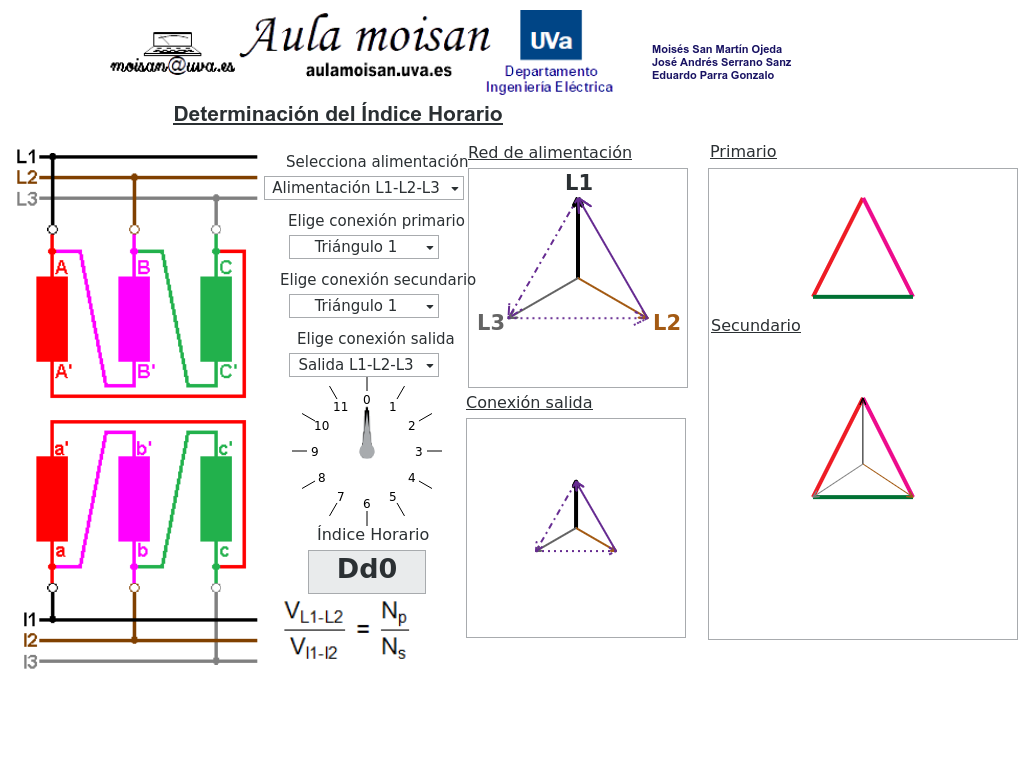
\includegraphics[width=0.7\textwidth]{images/fig_dd0.png}
    \caption{Simulación e índice horario resultante para la conexión Dd0.}
    \label{fig.ej2:dd0}
\end{figure}

\subsection{Configuración 2: Yy0}
Se configuró la conexión \textit{Estrella 1} tanto en el primario como en el secundario:
\begin{itemize}
    \item Primario: Bornes $A', B', C'$ cortocircuitados en el punto neutro; bornes $A, B, C$ de entrada.
    \item Secundario: Bornes $a', b', c'$ unidos en el neutro secundario; bornes $a, b, c$ de salida.
\end{itemize}
Dado que las estrellas de tensión primaria y secundaria se construyen de forma simétrica utilizando los mismos terminales
como neutro, las tensiones de fase secundaria se encuentran alineadas con sus correspondientes del primario. El desfase
resulta nulo ($0^\circ$), lo que da lugar al índice horario 0. Esta disposición y los correspondientes vectores resultantes
se ilustran en la figura~\ref{fig.ej2:yy0}.

\begin{figure}[!ht]
    \centering
    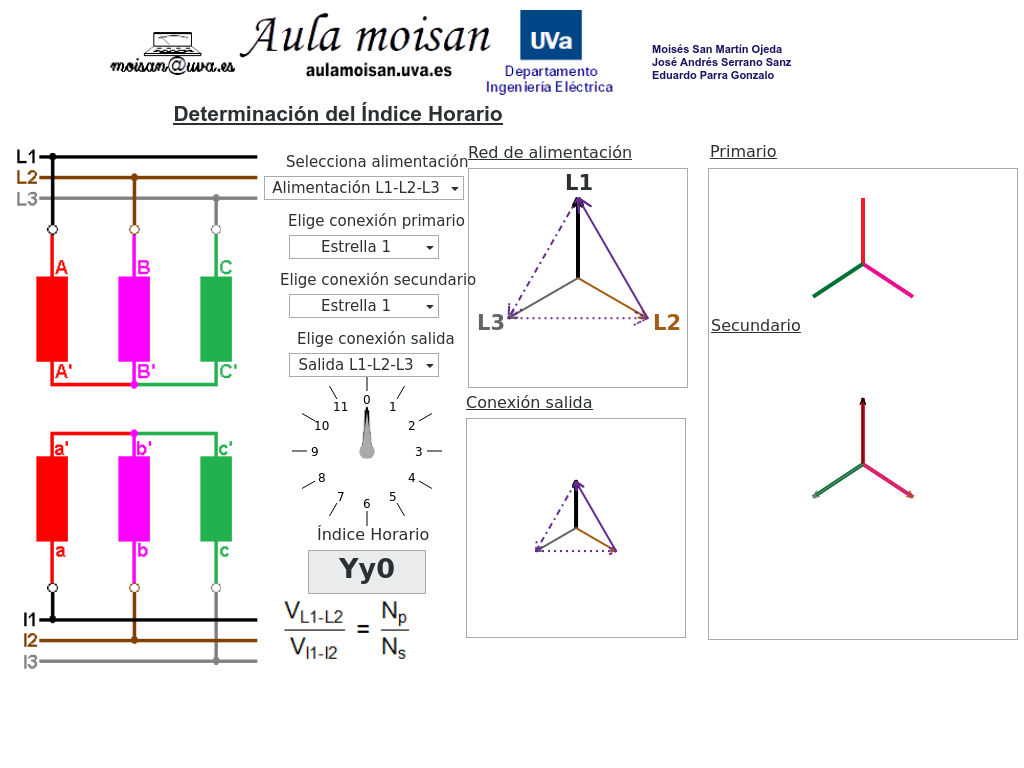
\includegraphics[width=0.7\textwidth]{images/fig_yy0.png}
    \caption{Simulación e índice horario resultante para la conexión Yy0.}
    \label{fig.ej2:yy0}
\end{figure}

\subsection{Configuración 3: Dz0}
En esta simulación se utilizó la conexión primaria \textit{Triángulo 1} y secundaria \textit{Zigzag 1}. Las conexiones
del secundario se realizaron de modo que:
\begin{itemize}
    \item Las mitades de los devanados $a1', b1', c1'$ forman el neutro común.
    \item Se conectan $a1-c2'$, $b1-a2'$ y $c1-b2'$.
    \item Las salidas del transformador se toman de los terminales libres $a2, b2, c2$.
\end{itemize}
La composición vectorial de la tensión del secundario sumando los dos semidevanados desfasados $120^\circ$ da como resultado
vectores de tensión de línea secundarios en fase con las tensiones compuestas del primario. De este modo, la superposición
de diagramas revela un desfase angular de $0^\circ$, determinando el índice horario 0. El comportamiento fasorial y la
configuración correspondiente se muestran en la figura~\ref{fig.ej2:dz0}.

\begin{figure}[!ht]
    \centering
    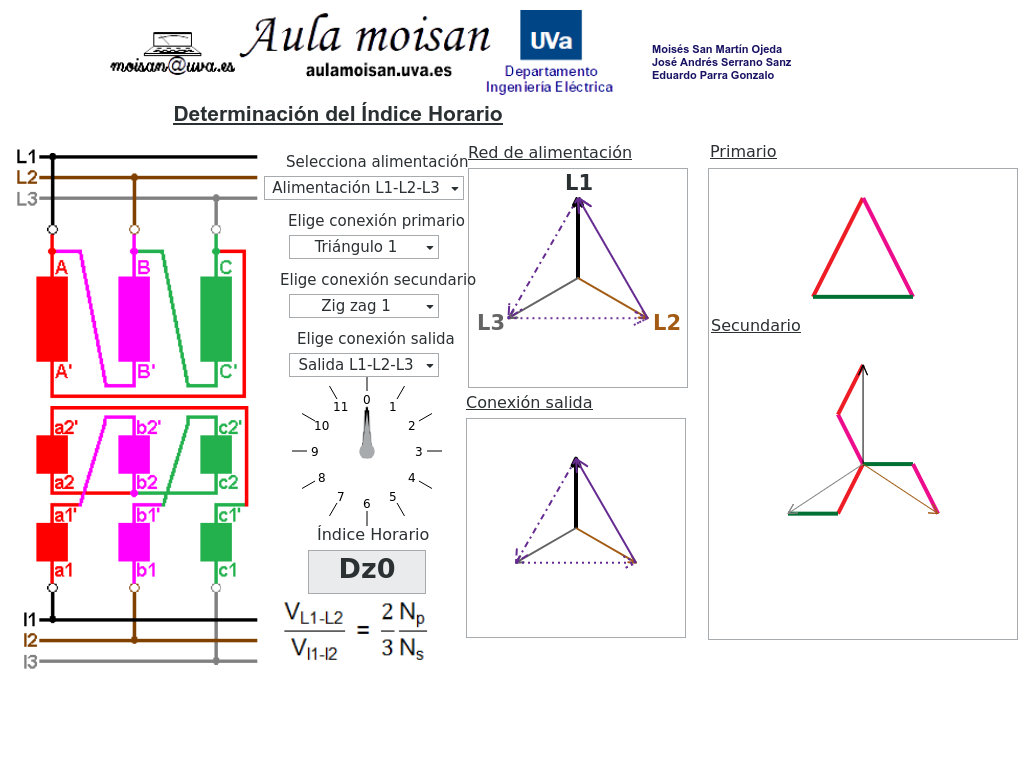
\includegraphics[width=0.7\textwidth]{images/fig_dz0.png}
    \caption{Simulación e índice horario resultante para la conexión Dz0.}
    \label{fig.ej2:dz0}
\end{figure}

\subsection{Configuración 4: Dy5}
Se configuró una conexión primaria del tipo \textit{Triángulo 2} y una conexión secundaria del tipo \textit{Estrella 2}.
Las conexiones se definen por:
\begin{itemize}
    \item Primario (\textit{Triángulo 2}): $A-B'$, $B-C'$ y $C-A'$. Esta alternancia desplaza los vectores del primario.
    \item Secundario (\textit{Estrella 2}): Los bornes $a, b, c$ forman el neutro; las salidas de línea se toman de $a', b', c'$.
\end{itemize}
La inversión del neutro en el secundario (estrella invertida respecto a la de tipo 1) genera un cambio de polaridad de $180^\circ$.
Al componer vectorialmente la estrella secundaria y superponerla al triángulo primario desplazado, se obtiene un desfasaje
angular neto de retraso de $150^\circ$, que equivale a la posición de las 5 horas en el reloj. La representación fasorial
de esta conexión en el simulador se presenta en la figura~\ref{fig.ej2:dy5}.

\begin{figure}[!ht]
    \centering
    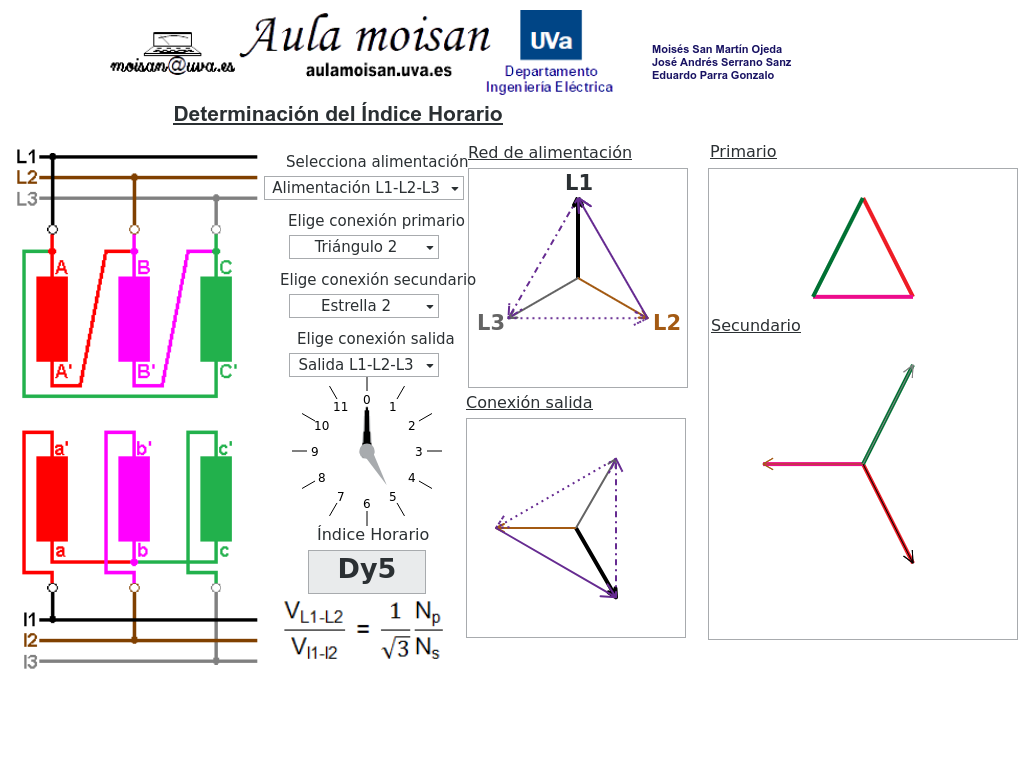
\includegraphics[width=0.7\textwidth]{images/fig_dy5.png}
    \caption{Simulación e índice horario resultante para la conexión Dy5.}
    \label{fig.ej2:dy5}
\end{figure}

\subsection{Configuración 5: Yd5}
Se configuró el primario en \textit{Estrella 2} y el secundario en \textit{Triángulo 1}:
\begin{itemize}
    \item Primario: Bornes $A, B, C$ unidos para formar el neutro; bornes $A', B', C'$ de entrada.
    \item Secundario: Conexión de triángulo clásica tipo 1 ($a'-b$, $b'-c$ y $c'-a$).
\end{itemize}
La conexión estrella del primario tiene la polaridad invertida en comparación con la estrella tipo 1, aportando un desfase
de $180^\circ$. Esto, en combinación con el desfasaje natural de $30^\circ$ de la conexión triángulo secundaria, resulta en
un ángulo de desfase de $150^\circ$ de retraso, correspondiente al índice horario 5. Este comportamiento fasorial y las
conexiones correspondientes pueden observarse en la figura~\ref{fig.ej2:yd5}.

\begin{figure}[!ht]
    \centering
    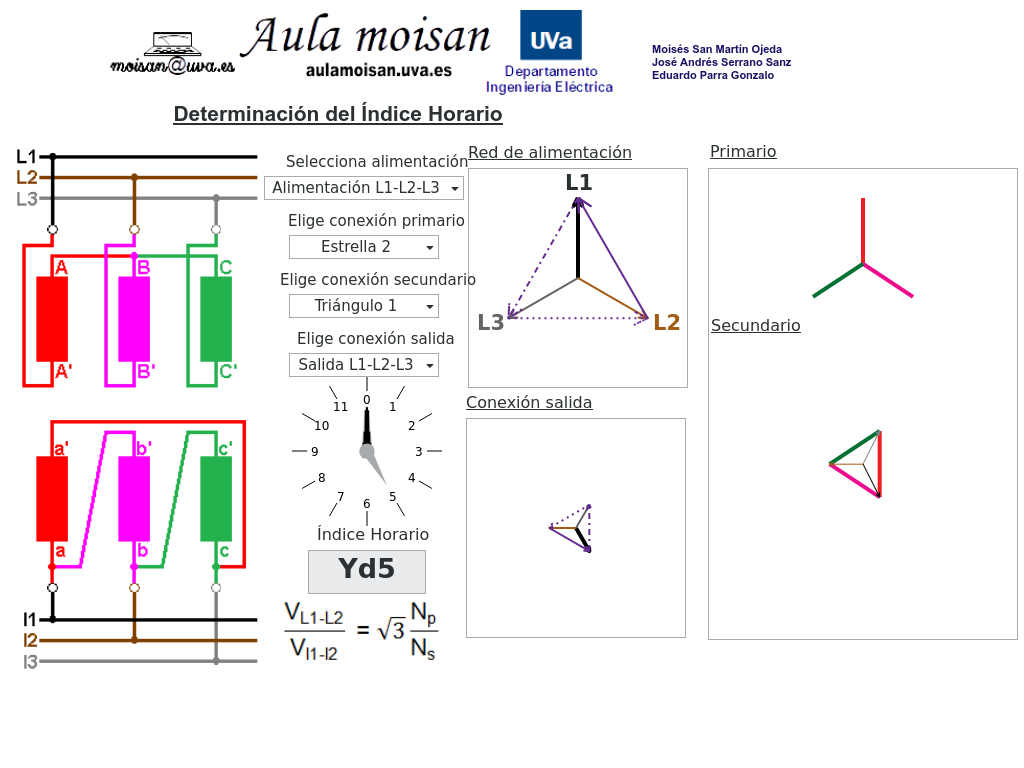
\includegraphics[width=0.7\textwidth]{images/fig_yd5.png}
    \caption{Simulación e índice horario resultante para la conexión Yd5.}
    \label{fig.ej2:yd5}
\end{figure}

\subsection{Configuración 6: Yz5}
Se empleó la conexión primaria en \textit{Estrella 2} y la conexión secundaria en \textit{Zigzag 1}. La inversión de la estrella
primaria introduce un desfase de $180^\circ$ en los vectores con respecto al neutro. Al componer vectorialmente la
tensión secundaria en zigzag y superponer los fasores, el vector secundario resultante se sitúa a un ángulo de $150^\circ$
de retraso con respecto al primario de referencia, marcando las 5 horas en el reloj. El diagrama de tensiones y la interfaz
del simulador para este ensayo se exhiben en la figura~\ref{fig.ej2:yz5}.

\begin{figure}[!ht]
    \centering
    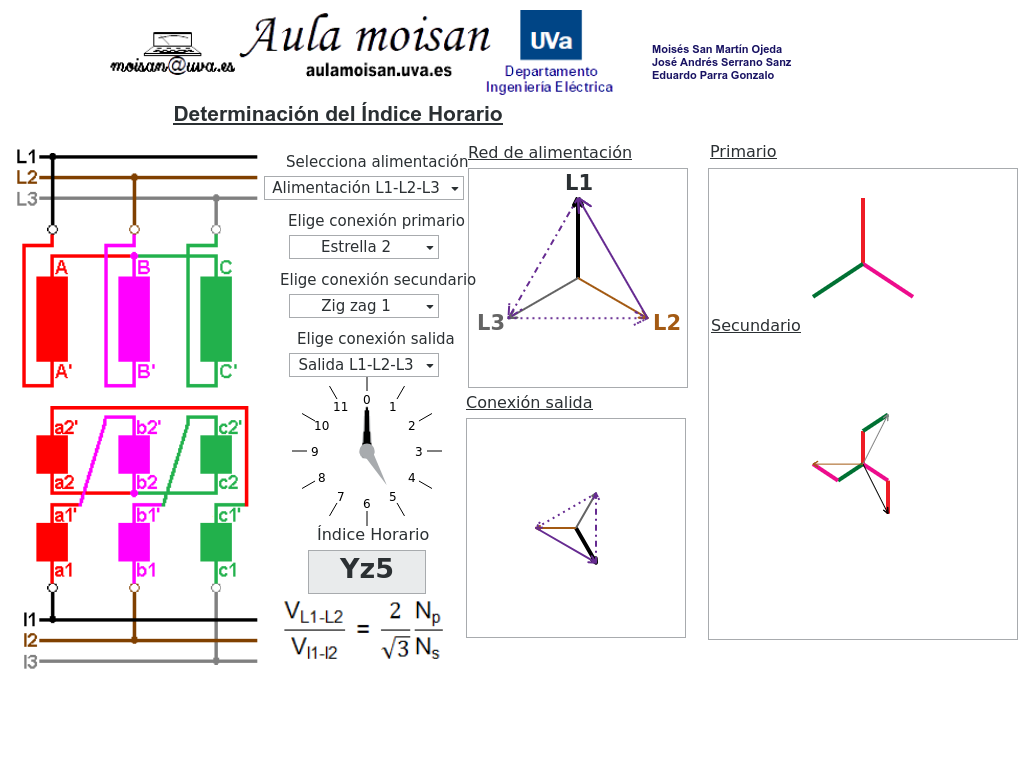
\includegraphics[width=0.7\textwidth]{images/fig_yz5.png}
    \caption{Simulación e índice horario resultante para la conexión Yz5.}
    \label{fig.ej2:yz5}
\end{figure}

\subsection{Configuración 7: Yy6}
Esta configuración utiliza la combinación de \textit{Estrella 2} en el primario y \textit{Estrella 1} en el secundario.
Dado que la estrella primaria tiene el neutro formado por los terminales sin prima ($A, B, C$) y la secundaria por los
terminales con prima ($a', b', c'$), se genera una inversión completa de polaridad en la representación vectorial de las tensiones
secundarias con respecto a las primarias. El desfase angular resultante es de $180^\circ$, marcando las 6 horas en la
esfera del reloj, lo que corresponde al índice horario 6. Los vectores opuestos y la configuración de terminales resultante
se aprecian en la figura~\ref{fig.ej2:yy6}.

\begin{figure}[!ht]
    \centering
    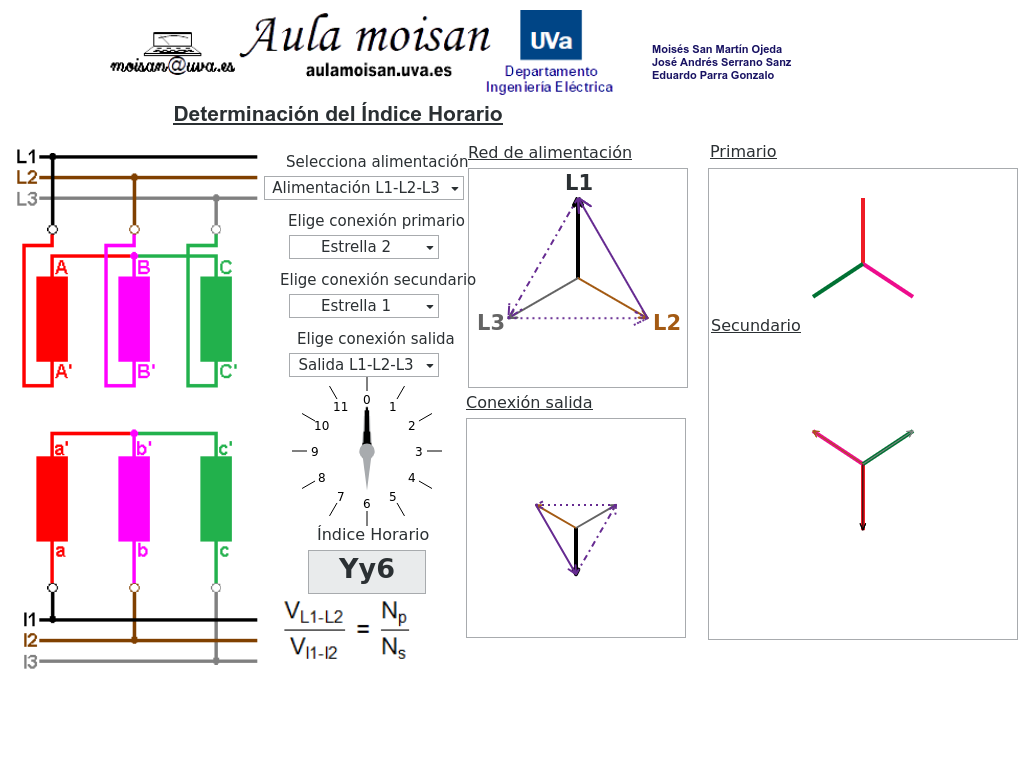
\includegraphics[width=0.7\textwidth]{images/fig_yy6.png}
    \caption{Simulación e índice horario resultante para la conexión Yy6.}
    \label{fig.ej2:yy6}
\end{figure}

\subsection{Configuración 8: Dz6}
Se configuró la conexión primaria en \textit{Triángulo 1} y secundaria en \textit{Zigzag 3}. Las conexiones secundarias para
el zigzag tipo 3 se realizaron de la siguiente forma:
\begin{itemize}
    \item Los bornes $a2, b2, c2$ se unen para formar el punto neutro secundario.
    \item Se conectan $a2'-b1$, $b2'-c1$ y $c2'-a1$.
    \item Las salidas del secundario se obtienen de los terminales $a1', b1', c1'$.
\end{itemize}
Esta disposición de bobinados y la toma de salida desde los terminales con prima de los semidevanados de base invierte los
fasores resultantes en comparación con el zigzag tipo 1. El desfase vectorial resultante respecto al triángulo del primario
es de $180^\circ$, de modo que el vector de baja tensión apunta a las 6 horas del reloj (índice 6). Esta inversión fasorial
de la tensión secundaria respecto al primario se detalla en la figura~\ref{fig.ej2:dz6}.

\begin{figure}[!ht]
    \centering
    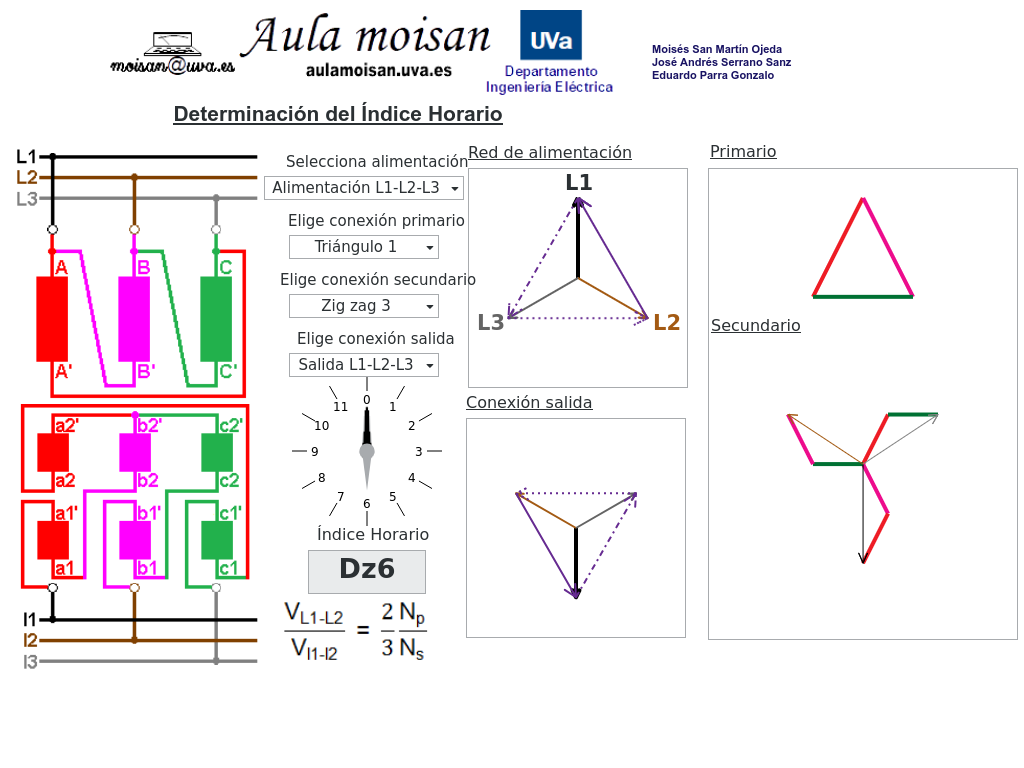
\includegraphics[width=0.7\textwidth]{images/fig_dz6.png}
    \caption{Simulación e índice horario resultante para la conexión Dz6.}
    \label{fig.ej2:dz6}
\end{figure}

\subsection{Configuración 9: Yz11}
Se utilizó una conexión del primario en \textit{Estrella 2} y del secundario en \textit{Zigzag 3}.
\begin{itemize}
    \item El primario está invertido (estrella tipo 2), introduciendo una rotación de $180^\circ$.
    \item El secundario está conectado en zigzag tipo 3, lo cual también invierte los fasores del secundario.
\end{itemize}
Al superponer ambos diagramas, los desfases de $180^\circ$ en ambos lados y la combinación intrínseca de los devanados
dan lugar a que la tensión de fase de baja tensión adelante $30^\circ$ a la de alta tensión. En sentido horario (de retraso),
esto equivale a un desfase de $330^\circ$, marcando las 11 horas en el reloj y configurando el índice 11. La compensación
vectorial resultante y los diagramas fasoriales se muestran en la figura~\ref{fig.ej2:yz11}.

\begin{figure}[!ht]
    \centering
    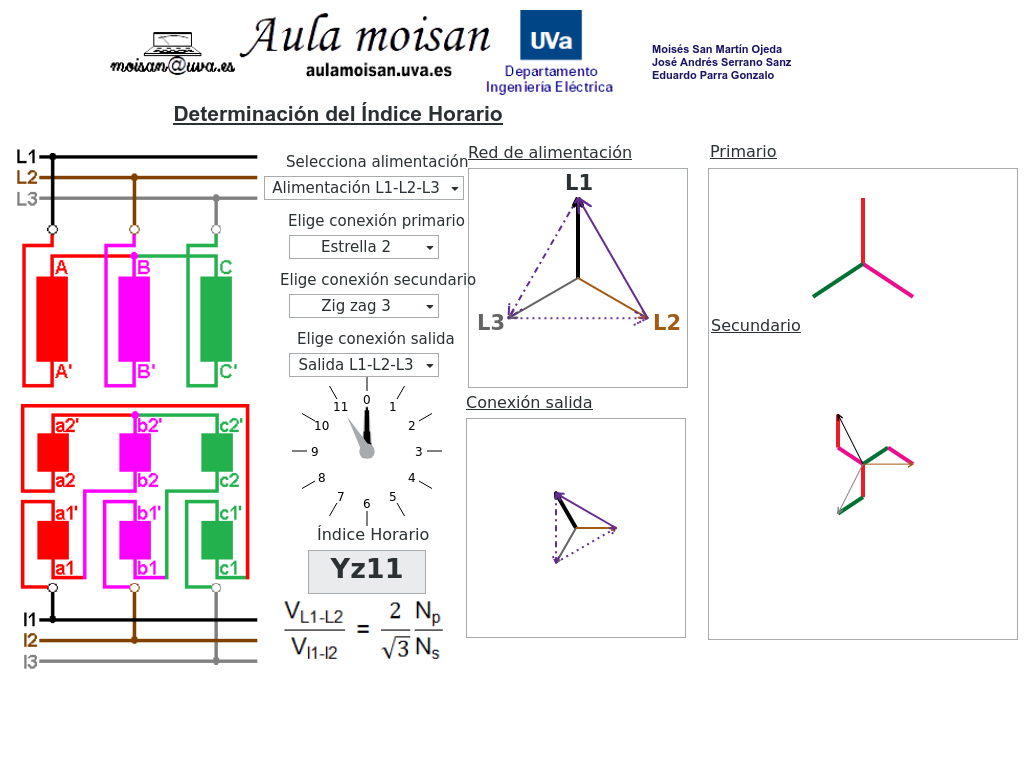
\includegraphics[width=0.7\textwidth]{images/fig_yz11.png}
    \caption{Simulación e índice horario resultante para la conexión Yz11.}
    \label{fig.ej2:yz11}
\end{figure}
